
\let\negmedspace\undefined
\let\negthickspace\undefined
\documentclass[journal]{IEEEtran}
\usepackage[a5paper, margin=10mm, onecolumn]{geometry}
%\usepackage{lmodern} % Ensure lmodern is loaded for pdflatex
\usepackage{tfrupee} % Include tfrupee package

\setlength{\headheight}{1cm} % Set the height of the header box
\setlength{\headsep}{0mm}     % Set the distance between the header box and the top of the text

\usepackage{gvv-book}
\usepackage{gvv}
\usepackage{cite}
\usepackage{amsmath,amssymb,amsfonts,amsthm}
\usepackage{algorithmic}
\usepackage{graphicx}
\usepackage{textcomp}
\usepackage{xcolor}
\usepackage{txfonts}
\usepackage{listings}
\usepackage{enumitem}
\usepackage{mathtools}
\usepackage{gensymb}
\usepackage{comment}
\usepackage[breaklinks=true]{hyperref}
\usepackage{tkz-euclide} 
\usepackage{listings}
\usepackage{gvv}                                        
\def\inputGnumericTable{}                                 
\usepackage[latin1]{inputenc}                                
\usepackage{color}                                            
\usepackage{array}  
\usepackage{longtable}                                       
\usepackage{calc}                                             
\usepackage{multirow}                                         
\usepackage{hhline}                                           
\usepackage{ifthen}                                           
\usepackage{lscape}
\usepackage{multicol}
\begin{document}

\bibliographystyle{IEEEtran}
\vspace{3cm}

\title{GATE-2011-AE}
\author{AI24BTECH11024-Pappuri Prahladha}
% \bigskip
{\let\newpage\relax\maketitle}

\renewcommand{\thefigure}{\theenumi}
\renewcommand{\thetable}{\theenumi}
\setlength{\intextsep}{10pt} % Space between text and floats


\numberwithin{equation}{enumi}
\numberwithin{figure}{enumi}
\renewcommand{\thetable}{\theenumi}
\begin{enumerate}[start=14]
 \item  In an un-powered glide of an aircraft having weight $W $, lift $ L $ and drag $ D $, the equilibrium glide angle is defined as
 \begin{multicols}{1}
    
    \begin{enumerate}
        \item  $\tan^{-1} \left( \frac{L}{D} \right)$ 
        \item  $\tan^{-1} \left( \frac{D}{L} \right)$ 
        \item  $\tan^{-1} \left( \frac{L}{W} \right) $
        \item  $\tan^{-1} \left( \frac{W}{L} \right) $
    \end{enumerate}
\end{multicols}  
\item  Lift on an aircraft climbing vertically up is
 \begin{multicols}{2}
    \begin{enumerate}
        \item equal to its weight
        \item zero
        \item equal to the drag
        \item equal to the thrust
    \end{enumerate}
\end{multicols}   
 \item If an aircraft is performing a positive yawing manoeuvre, the side slip angle
 \begin{multicols}{1}

    \begin{enumerate}
        \item is always zero
        \item is never zero
        \item is always negative
        \item could be any value
    \end{enumerate}
\end{multicols}
\item For an airplane to be statically stable, its centre of gravity must always be
 \begin{multicols}{2}
    \begin{enumerate}
        \item ahead of wing aerodynamic centre
        \item aft of the wing aerodynamic centre
        \item ahead of neutral point
        \item aft of neutral point
    \end{enumerate}
\end{multicols} 
 \item  It is seen that the drag polar of a certain aerofoil is symmetric about the $ C_{d} $ axis. This drag polar could refer to
 \begin{multicols}{1}
    \begin{enumerate}
        \item NACA 0012
        \item NACA 4415
        \item NACA 23012
        \item None of the above
    \end{enumerate}
\end{multicols}
\item The aerodynamic centre of a supersonic aerofoil, with chord $ c $, is located at
 \begin{multicols}{1}
    \begin{enumerate}
        \item the leading edge
        \item 0.25c 
        \item 0.5c 
        \item 0.75c 
    \end{enumerate}
\end{multicols}
\item Winglets are used on wings to minimize
 \begin{multicols}{1}
    \begin{enumerate}
        \item skin friction drag
        \item profile drag
        \item wave drag
        \item induced drag
    \end{enumerate}
\end{multicols}
\item Consider a potential flow with free stream velocity $ V_{\infty} $, over a spinning circular cylinder of radius  $R$  and circulation  $\Gamma$ . The stream function,  $\psi$ , where  $\psi = 0$  on the cylinder surface, in cylindrical coordinates  $\brak{r, \theta}$, is given by
 \begin{multicols}{2}
    \begin{enumerate}
        \item  $V_{\infty} r \cos \theta \brak{ 1 - \frac{R^2}{r^2} } + \frac{\Gamma}{2 \pi} \ln \frac{r}{R} $
        \item  $V_{\infty} r \cos \theta \brak{ 1 + \frac{R^2}{r^2} } + \frac{\Gamma}{2 \pi} \ln \frac{r}{R} $
        \item  $V_{\infty} r \sin \theta \brak{ 1 - \frac{R^2}{r^2} } + \frac{\Gamma}{2 \pi} \ln \frac{r}{R} $
        \item  $V_{\infty} r \sin \theta \brak{ 1 + \frac{R^2}{r^2} } + \frac{\Gamma}{2 \pi} \ln \frac{r}{R} $
    \end{enumerate}
\end{multicols}
\item A main objective of by-pass in a turbo-fan engine is to increase
 \begin{multicols}{2}
    \begin{enumerate}
        \item mass flow rate through engine inlet
        \item turbine inlet temperature
        \item mass flow rate through exhaust nozzle
        \item compressor pressure ratio
    \end{enumerate}
\end{multicols}
\item The pressure ratio in any one stage of a jet engine compressor is limited by
    \begin{enumerate}
        \item entry stagnation temperature in that stage
        \item entry Mach number in that stage
        \item pressure gradient induced separation in that stage
        \item mass flow rate in that stage
    \end{enumerate}

\item Thermodynamic cycle on which the jet engine operates can be
 \begin{multicols}{2}
    \begin{enumerate}
        \item open Rankine cycle only
        \item either open or closed Rankine cycle
        \item open Brayton cycle only
        \item either open or closed Brayton cycle
    \end{enumerate}
\end{multicols}
\item Propulsion efficiency of a jet engine is
    \begin{enumerate}
        \item directly proportional to both the thrust power and the air mass flow rate
        \item inversely proportional to both the thrust power and the air mass flow rate
        \item directly proportional to thrust power and inversely proportional to the air mass flow rate
        \item inversely proportional to thrust power and directly proportional to the air mass flow rate
    \end{enumerate}


\item  Consider a cantilever beam having length $ L = 1m $, square cross-section\\ (width = depth = 0.01 m) and Young's modulus 50 GPa. The beam is subjected to a transverse load $ P = 1N $ at the mid-span $\brak{L/2}{}$ at the center of the cross-section. Under the small deformation theory, the transverse deflection of the beam (in mm) at its free-end is \rule{3cm}{0.15mm}



 \begin{figure}[h!]
   \centering
   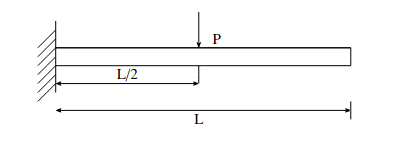
\includegraphics[width=0.7\linewidth]{figs/figure1.png}
   \label{stemplot}
\end{figure}

\end{enumerate}
\end{document}
